\newif\ifvimbug
\vimbugfalse

\ifvimbug
\begin{document}
\fi

\exercise{Linear Regression}

In this exercise, you will use the dataset \texttt{linRegData.txt}, containing $150$ points in the format \texttt{<input variable, output variable>}. The input is generated by a sinusoid function, while the output is the joint trajectory of a compliant robotic arm. 
The first 20 data points are the training set and the remainder are the testing set.

\begin{questions}

%----------------------------------------------

\begin{question}{Polynomial Features}{10}
Write the equation of the model and fit it with polynomial features. Using the Root Mean Square Error (RMSE) as a metric for the evaluation, select the complexity of the model (up to a 21st degree polynomial) by evaluating its performance on the testing data. Which is the best RMSE you achieve and what is the model complexity? Does it change if we evaluate our model on the training data? Comment your findings and plot the RMSE for each case (use two lines, one for evaluation on training data, one for evaluation on testing data).
For the estimation of the optimal parameters use a ridge coefficient of $\lambda=10^{-6}$.
\\Using what you think is the best learned model from the previous point, show in a single plot the ground truth (full dataset) and the model prediction over it.
Attach snippets of your code showing how you generate polynomial features and how you fit the model.

\begin{answer}\end{answer}

\end{question}

%----------------------------------------------

\begin{question}{Gaussian Features}{4}
Now use Gaussian features. Each feature is a Gaussian distribution were the means are distributed linearly in $x \in[0,2]$ and the variance is set to $\sigma^2=0.02$. The features have to be normalized, i.e., they have to sum to one at every $x$. Using 10 features generate a plot with the activation of each feature over time (i.e., plot the matrix $\Phi$). Attach a snippet of your code showing how to compute Gaussian features.

\begin{answer}\end{answer}

\end{question}

%----------------------------------------------

\begin{question}{Gaussian Features, Continued}{4}
Repeat the process of fitting the model using the Gaussian features from the previous question. Compare the RMSE on the testing data using $15 \ldots 40$ basis functions and plot the RMSE. Which number of basis functions has the best performance and what is the best RMSE? Use a ridge coefficient of $\lambda=10^{-6}$.

\begin{answer}\end{answer}

\end{question}

%----------------------------------------------

\begin{question}{Bayesian Linear Regression}{10}
Using Bayesian linear regression, plot the mean and the standard deviation of the predictive distribution learned using the first $\{10, 12, 16, 20, 50, 150\}$ data points (one plot per case; plot it in the interval $x\in[0,2]$).
Discuss how the model uncertainty changes with the amount of data points and the problem of overfitting with Bayesian linear regression.
Use the best performing polynomial features that you found in 3.1a, a ridge coefficient of $\lambda=10^{-6}$, and assume Gaussian noise with $\sigma^2=0.0025$. 

\begin{answer}\end{answer}
\end{question}

%----------------------------------------------

\begin{question}[bonus]{Cross Validation}{5}
So far, we have split our dataset in two sets: training data and testing data. Cross-validation is a more sophisticated approach for model selection. Discuss it and its variants, pointing out their pro and cons.
\end{question}


Cross validation is used for a number of different techniques in machine learning. In general it means comparing a Trainingset with some kind of Validation or Testset. Using this definition the easiest crossvalidation-method is the holdout method. The holdout method splits the data into three sets: Training-, Validation and Testset. The machine learning Algorithm is trained using the training set and evaluated on the validation set, for tweaking the parameters\ref{fig:holdout}. This approach prevents knowledge "leaking" from the Testset into the model. Therefore the metrics used on the testing set will measure the ability of the model to generalize. 
\begin{figure}[H]
	\includegraphics[width=0.7\linewidth]{pictures/holdout.png}
	\centering
	\caption{Holdout Cross-Validation schematic}
	\label{fig:holdout}
\end{figure}



While simple, this approach comes with several limitations. Mainly in reducing the number of training samples for learning the model drastically, but also for introducing a high amount of variance in the evaluation, since the results can depend on a particular random choice of train and validation sets. 

To solve this problem k-fold crossvalidation (often just cross-validation, cv) is used. A test set still needs to be hold out for final validation, but we dont need a seperate validation set anymore. Instead we split the training set in \textit{k} smaller sets. The model is now trained on k-1 sets and validated on the remaining part. This process is now repeated for each of the "k-folds" \ref{fig:holdout}.

\begin{figure}[H]
	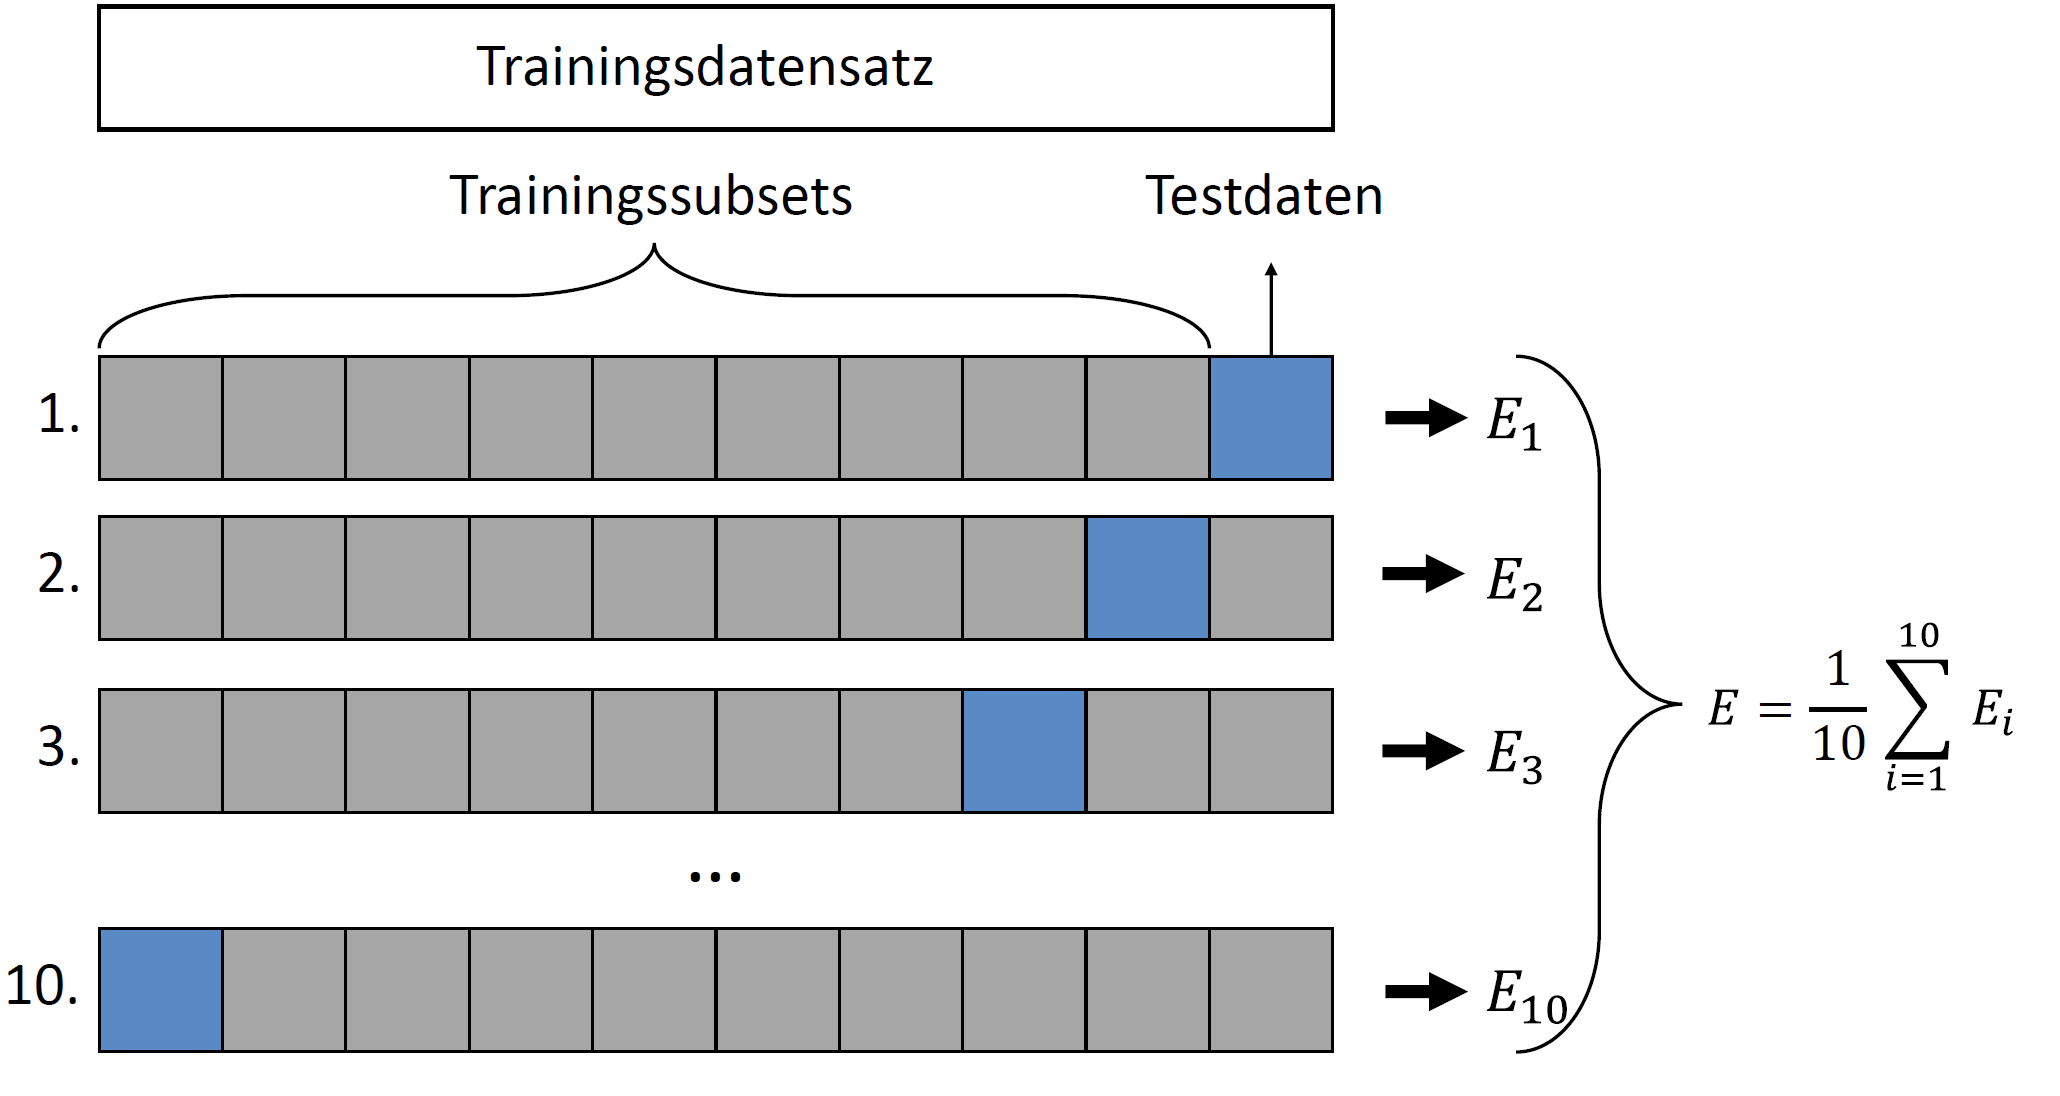
\includegraphics[width=0.7\linewidth]{pictures/cross_validation.png}
	\centering
	\caption{k-Fold cross validation splits the data into k-sets.}
	\label{fig:cv}
\end{figure}

The measured perfromance is the average of all individuall runs. This approach can be quite expensive to compute, but uses less data and generally leads to less variance in the outcome. 

To futher reduce the variance one can use the stratified k-fold cross-validation method. This method can be used, whenever all data is seen as equally important by the estimator, but may not be in reality. Instead of random shuffling the datasets, the stratified approach tries to create "stratified" folds, meaning that all folds have about the same percentage of samples of each target class, as the complete set. Only works on classification problems. 

K-fold cross-validation reaches its limiations when one wants to Hyperparameterize their models. Since no validation set is used, any change of parameters done after seeing the test metrics will lead to overfitting. To bypass this, nested cross-validation is used. In nested cross-validation another loop is added to the process, to be able to hyperparameterize algorithms. Now the inner cross-validation loop is used for training and validating models, while the outer loop is used for changing hyperparameters (for example by using grid search) and to evaluate different model architectures. For example, when using nested cross-validation with neural networks, the inner loop is used to train the network by changing its weights and bias vectors and validate its generalizing performance. Meanwhile the outer loop will be used for changing its hyperparameters e.g. the number of hidden layers and Neurons. The result of the outer loop leads to the best overall model. The excact process is shown in the picture \ref{fig:ncv}.

\begin{figure}[H]
	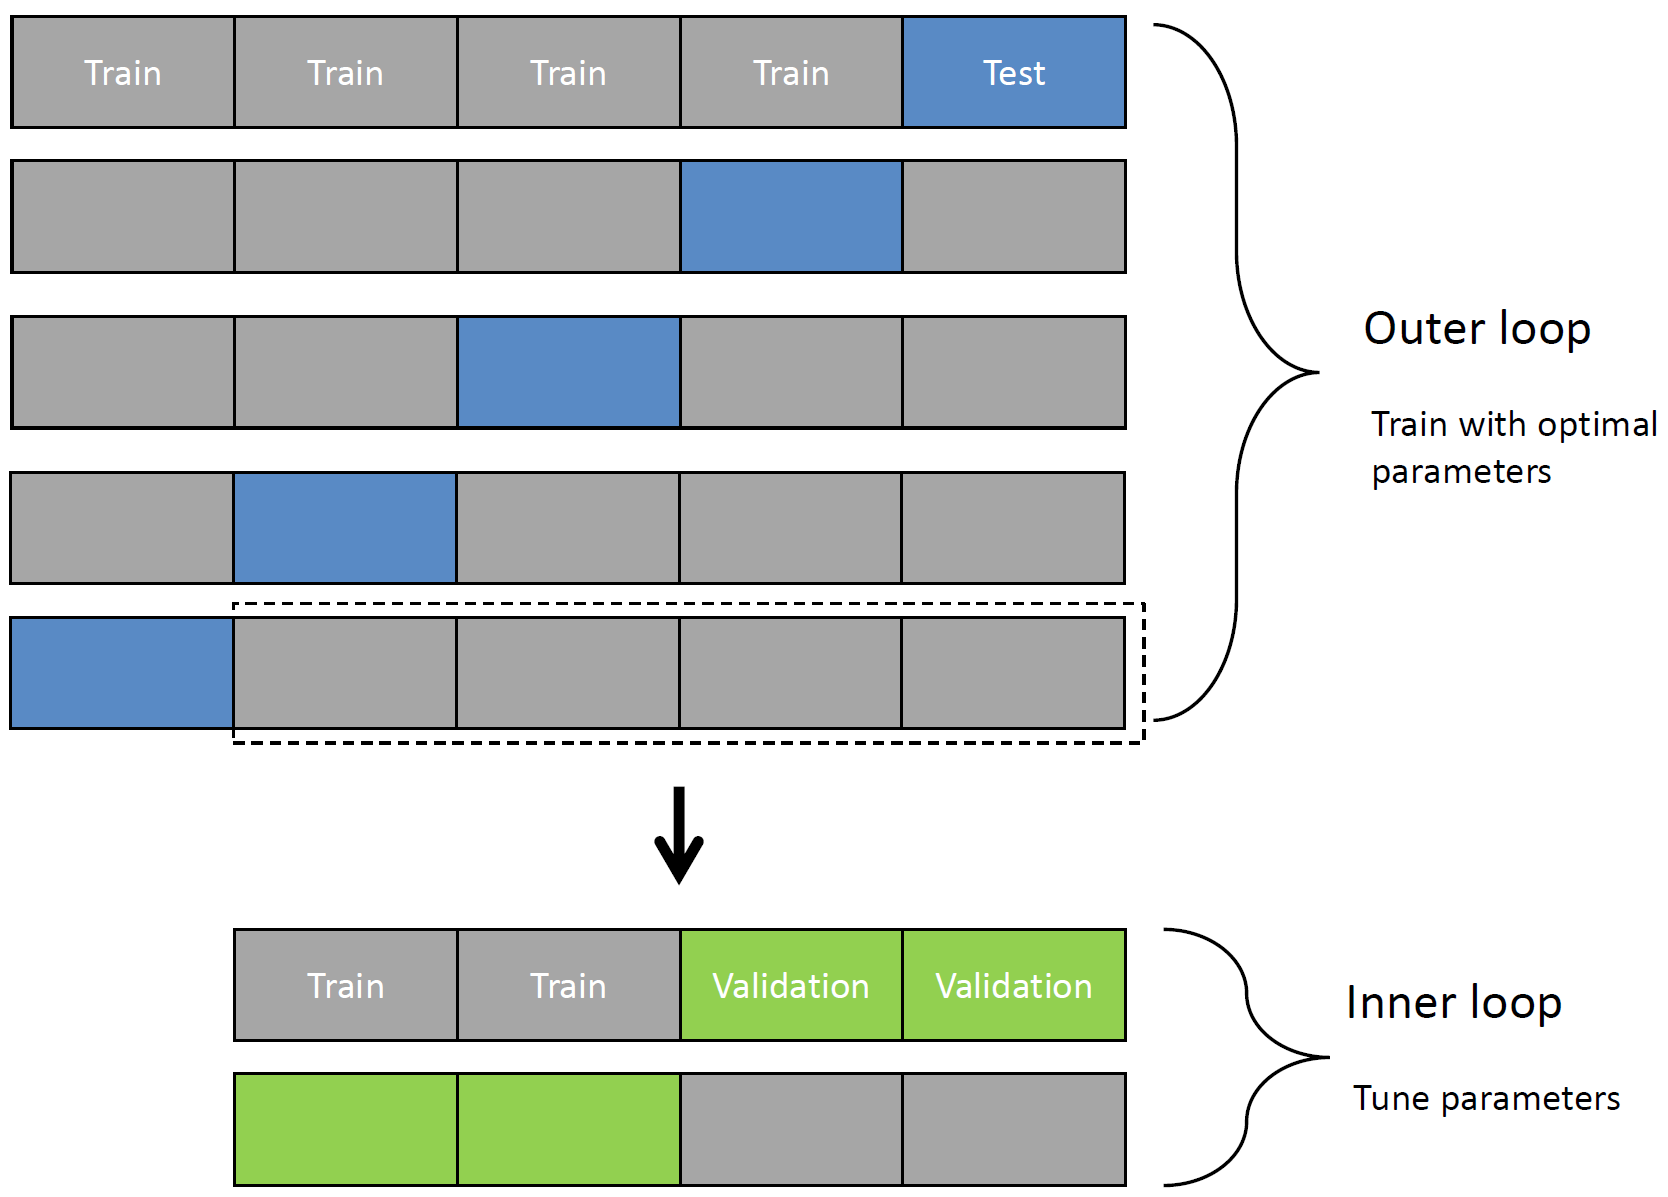
\includegraphics[width=0.8\linewidth]{pictures/nested_cross_validation.png}
	\centering
	\caption{Schematic of nested cross validation. The inner loop is used to train and validate a simple mode, while the outer loop is used to compare different model architecures.}
	\label{fig:ncv}
\end{figure}

\begin{answer}
\end{answer}

\end{questions}
